\section*{Results}

\subsection*{Adjacency matrix, list generation}

\begin{lstlisting}[caption=1-2 lines of adjacency matrix, label=lst:1]
    [
        [0, 0, 0, 0, 0, 0, 0, 0, 0, 0, 0, 0, 0, 0, 0, 0, 0, 0, 0, 0, 0, 0, 0, 0, 0, 0, 0, 0, 0, 0, 0, 0, 0, 0, 0, 0, 0, 0, 0, 0, 0, 0, 0, 0, 0, 0, 0, 0, 0, 0, 0, 0, 0, 0, 0, 0, 0, 0, 0, 0, 0, 0, 0, 0, 0, 0, 0, 0, 0, 0, 1, 0, 0, 0, 0, 0, 0, 0, 0, 0, 0, 0, 0, 0, 0, 0, 0, 0, 0, 0, 0, 1, 0, 0, 0, 0, 0, 0, 0, 0], 
        [0, 0, 0, 0, 0, 0, 0, 0, 0, 0, 0, 0, 0, 0, 0, 0, 0, 0, 0, 0, 0, 0, 0, 0, 0, 0, 0, 1, 0, 0, 0, 0, 1, 0, 0, 0, 0, 0, 0, 0, 0, 0, 0, 0, 0, 0, 0, 0, 0, 0, 0, 0, 0, 0, 0, 0, 0, 0, 0, 0, 0, 0, 0, 0, 0, 0, 0, 0, 0, 0, 0, 0, 0, 1, 0, 0, 0, 0, 0, 0, 0, 0, 0, 0, 0, 0, 0, 0, 0, 0, 0, 0, 0, 0, 0, 0, 0, 0, 0, 0], 
    ]
\end{lstlisting}

\begin{lstlisting}[caption=Adjacency for 1-2 vertices, label=lst:2]
    [[91, 70], [27, 73, 32]]
\end{lstlisting}

In listings \ref{lst:1}, \ref{lst:2} two possible representation of graphs: Adjacency matrix, Adjacency list are shown.
As it seen the Adjacency list is much more compact for graph observed in the work due to its sparse form. It can be concluded that adjacency list is more efficient in terms of memory consumption in case of sparse graphs.
It requires $O(|E| + |V|)$ of space while adjacency matrix $O(|V|^2)$.

As well as that adjacency list is more convient for implementing DFS and BFS algorithms due to ability traverse only vertices that adjecent to observed one. On the other testing the connectivity between 2 vertices can be done more efficient by means of adjacency matrix in time of $O(1)$.

\begin{center}
    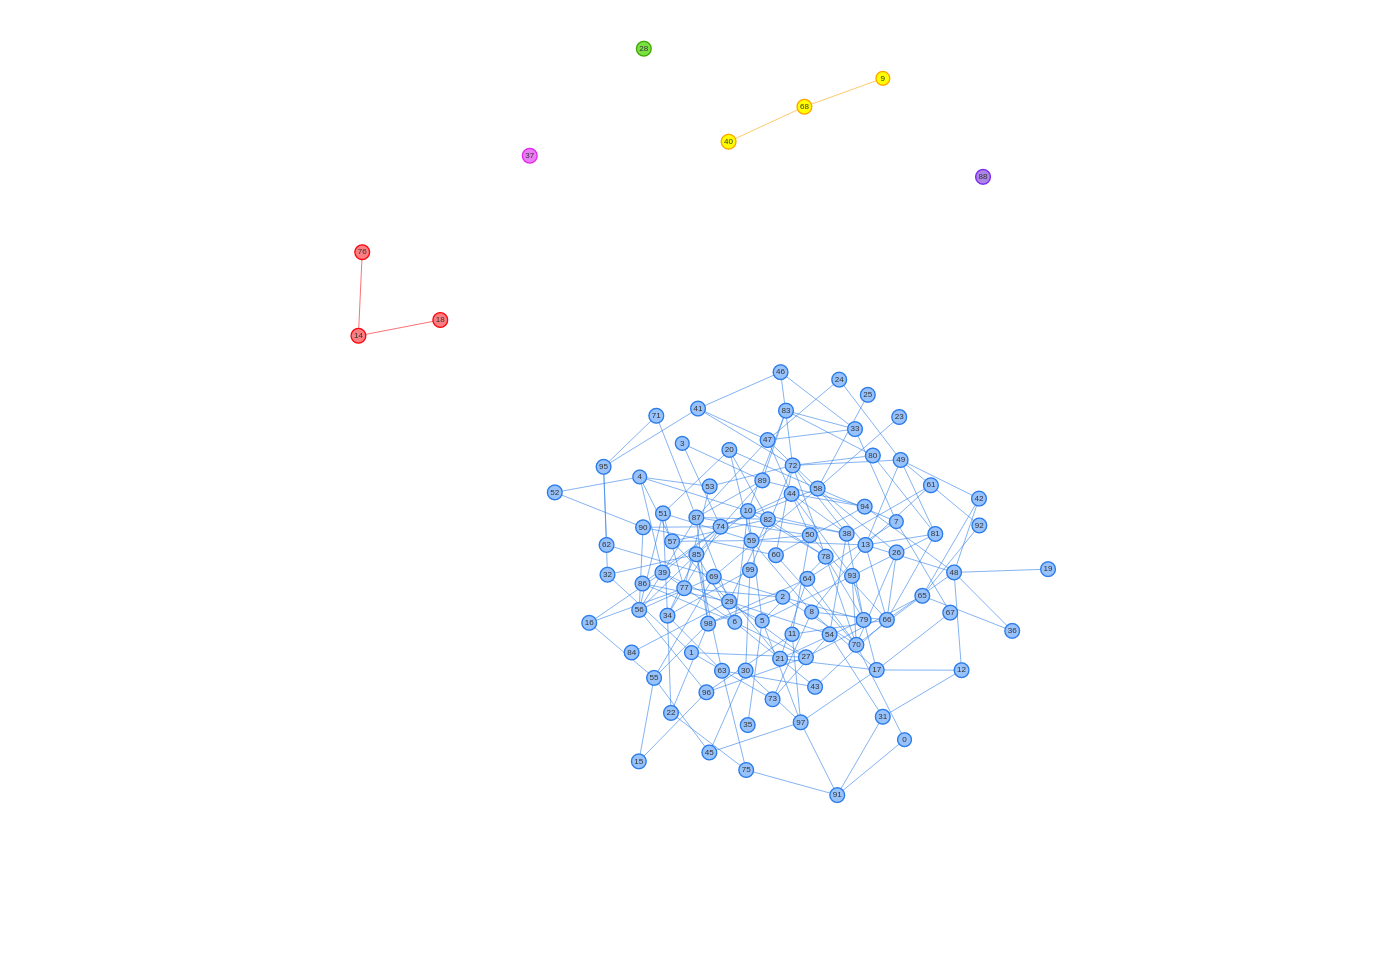
\includegraphics[width=\linewidth]{../results/grapht.png}
    \captionof{figure}{Graph with separeted in connectivity components}
    \label{fig:dfs_result}
\end{center}

\subsection*{DFS, BFS algorithms}

In the Figure \ref{fig:dfs_result} generated graph is shown. Different connectivity components are shown in different colours. To obtain components the Depth-first search algorithm was used.
It was ran from every unseen vertix while counting the number of such runs - connectivity component count = 6.

\begin{center}
    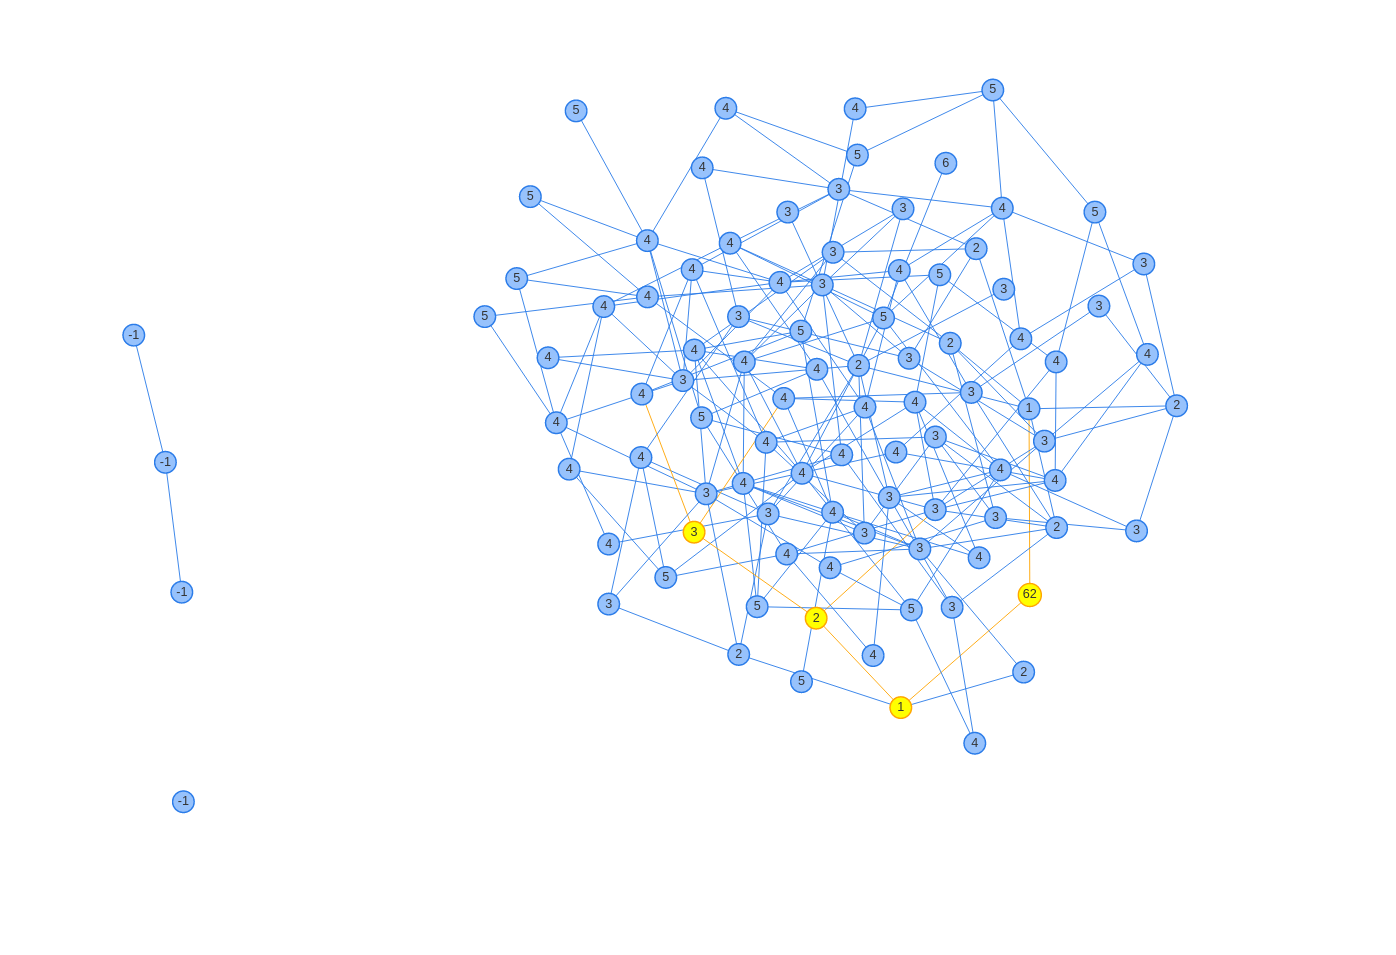
\includegraphics[width=\linewidth]{../results/bfs_result.png}
    \captionof{figure}{Result of Breadth-first search}
    \label{fig:bfs_result}
\end{center}

In the Figure \ref{fig:bfs_result} the result of running Breadth-first search from vertex with number 62 is visualized.
Labels of other vertex shows obtained distance from original vertex. Label value $-1$ means that vertex is not connected to start one and belongs to another connectivity component.

In yellow showed vertices on the path from 62th to 1st vertix: 62, 95, 32, 1. The length of path is 3 as it seen in figure. 

\subsection*{Used data-structures}

Originally, the graph was generated in form of edges list of length 200 as a subset of all possible edges (that are present in complete graph).
After that it was converted to adjacency matrix and adjacency list. The later was used in implementation of DFS and BFS algorithms.

In BFS algorithm the deque data-strucute was used as an implementation of FIFO interface for processing queueing vertices.